\documentclass[12pt,a4paper]{article}
\usepackage[top=2cm, bottom=2cm, left=2cm, right=2cm]{geometry}

\usepackage{amsmath}
\usepackage{amsfonts}
\usepackage{amssymb}
\usepackage{graphicx}

\usepackage{fontspec}
\setmainfont{Arial}

\usepackage[style=ieee]{biblatex}
\addbibresource{evco.bib}

\usepackage{listings}
\usepackage{longtable}
\usepackage{tabu}
\usepackage{multirow}
\usepackage{subcaption}


\usepackage{hyperref}
\hypersetup{
	colorlinks=true,       % false: boxed links; true: colored links
	allcolors=blue
}

\begin{document}
	
	\begin{titlepage}
		\begin{center}
		\textbf{MEng/MMath/MSc Degree Examinations 2017/18}
		
		\textsc{DEPARTMENT OF COMPUTER SCIENCE}
		
		\vspace{3cm}
		
		\Large
		\textbf{Evolutionary Computation (EVCO)
		Individual Assessment}
	
		\vspace{1.5cm}
		
		\large
		\textbf{Examination Number: Y1403115}
		\end{center}
	\end{titlepage}
	
	
	% 2) Introduction [15 marks]
	\section{Introduction}
	%Intro
	Snake is a 2D, single player action game. The goal of the game is to navigate a snake through a grid, collecting as many food items as possible. The snake's length grows with each eaten food item. The game is over whenever the snake hits its own body or the wall (in the version of the games where there are walls). 
	
	In this report, a genetic programming (GP) approach is presented for evolving an intelligent snake agent, which aims to achieves as high a score as possible. GP has been proven successful in producing intelligent game agents for several games (\cite{ehlis_application_2000}, \cite{cole_using_2004}, \cite{shichel_gp-robocode:_2005}, \cite{koza_genetic_1992}).
	
	The report is structured as follows: \autoref{related_work} presents related work in evolutionary algorithms (EA) for games, as well as heuristic and evolutionary approaches for solving the snake game. \autoref{methods} describes the problem and particular approach used to find a solution. \autoref{results} discusses the results obtained from experiments. And \autoref{conclusions} summarises the findings and suggests further work.
	
	\subsection{Realated work} \label{related_work}
	%Game playing EA
	In the literature, there are many examples of using evolutionary algorithms to produce intelligent game playing agents. Some of the applications include using EAs to find optimal parameters for game controllers: Pac-Mann \cite{gallagher_learning_2003}, The Open Racing Car Simulator (TORCS) video game \cite{munoz_multi-objective_2010} and Counter Strike \cite{cole_using_2004}; using EA based optimisation to find a game state weighting function: Tetris \cite{bohm_evolutionary_2018}; using genetic programming to design a controller for Robocode \cite{shichel_gp-robocode:_2005}; and using neuroevolution approach to produce agents that play a variety of Atari 2600 games  \cite{hausknecht_neuroevolution_2014}.
	
	%Snake playing AI
	Even though there is interest in applying EAs to games in general, there is not much research done in using EAs for the snake game. Kong et. al. \cite{kong_automated_nodate} compares different search algorithms none of which uses EAs. Their findings show the algorithms that perform slower have greater reliability in terms of the snake not crashing before it has eaten all the food. 
	
	Yeh et. al. \cite{yeh_snake_2016} propose a snake controller, which uses a weighted sum of rating functions to determine the best move at each time step. The rating functions are smoothness (number of subsequent moves in the particular direction), space (how many squares can be reached) and distance to food. An EA is used to determine the weights for each rating function. The controllers are evolved in a game environment with fixed food positions. They outperformed a heuristic based approach in the same game environment, However this is not true in a game with random food positions.
	
	Ehlis \cite{ehlis_application_2000} uses GP to find a routine, consisting of the snakes sensing and movement functions, which achieves the maximum score. This approach is very similar to the solution of the Santa Fe Ant problem described in \cite{koza_genetic_1992} because it uses the game agent's sensors and actuators directly as a function set in the GA. The paper focuses on finding a function set, which results in the best performance.
	

	% 3) Methods [35 marks]
	\section{Methods} \label{methods}
	
	\subsection{Problem analysis}
	The game environment is a 14 by 14 grid of squares, with walls in all squares with indexes 0 or 13. The snake starts in square (4,10) and its initial length is 11. On each time step the snake moves one square in the direction it is facing. The snakes action allow it to turn (in place) in one of four direction - up, down, right, left. The directions are defined relative to the grid and not the snake's direction of movement. When the snake "eats" a food item, a new one is placed at random on a square, which is not occupied by the snake's body. The game ends whenever the snake enters a square, which has a wall or the snake's body in it, or if the snake makes 196 moves without eating any food.  
	
	The GP approach used for the snake game was motivated by Ehlis \cite{ehlis_application_2000} as well as the solution to the Santa Fe Ant problem described in \cite{koza_genetic_1992} and implemented in \cite{noauthor_artificial_nodate}. However, there are some subtle differences between these two problems and the snake game. In particular, the turning actions of the snake are defined in terms of the global directions and not the direction, the snake is facing. This means that the snake can potentially turn at 180 degrees, facing its own body and collide with it. This makes the game harder, as there is always a danger in one of the squares adjacent to the snakes head. 
	
	It is worth reasoning about which agent behaviour is desirable and which solutions are optimal. A simple optimal solution to the snake game is a Hamiltonian circuit \cite{noauthor_hamiltonian_2017} - a path going through all squares of the grid irrespective of where the food is. This way wherever the food appears, the snake will eventually eat it because it is traversing every single square. Ehlis \cite{ehlis_application_2000} reports that all optimal solutions found follow some Hamiltonian path.
	
	Some important qualities for successful agents include avoiding walls, avoiding own body, avoiding dead ends. Furthermore, if the snake agent is not following a Hamiltonian path it is important for it to aim for the food before the timer runs out.
	
	\begin{figure}[h!]
		\centering
		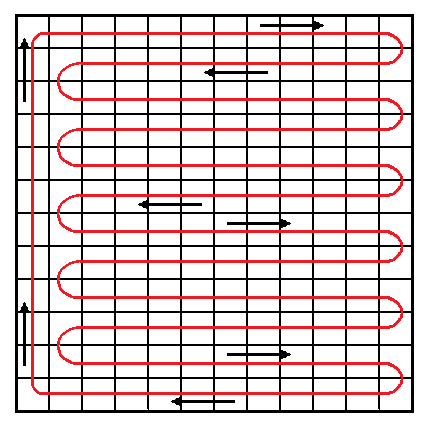
\includegraphics[width=0.7\linewidth]{figures/hamiltonian}
		\caption{Snake game hamiltonian path}
		\label{fig:ham_path}
	\end{figure}
	
		
	\subsection{Choice of representation}
	Each individual in the GP algorithm is represented as a tree of operations from a function set. The function set comprises of terminal and non-terminal nodes. The terminal nodes are the movement functions of the snake, which don't have any input parameter or outputs, but just change the direction of the snake. The non-terminals are the sensing functions of the snake and all take as inputs two other functions (terminals or non-terminals) and depending on the evaluation of a certain condition, execute one of them. For example, an individual, who turns right whenever there is food in the square, right of the snake's head, is shown in \autoref{fig:tree}. The tree is equivalent to the python expression \lstinline|if_food_right(changeDirectionRight, changeDirectionUp)|, which executes \lstinline|changeDirectionRight| if there is food in the right square and \lstinline|changeDirectionUp| otherwise. 
	
	The terminal function set is shown in \autoref{table:terminals}. 
	
	\begin{figure}[h!]
		\centering
		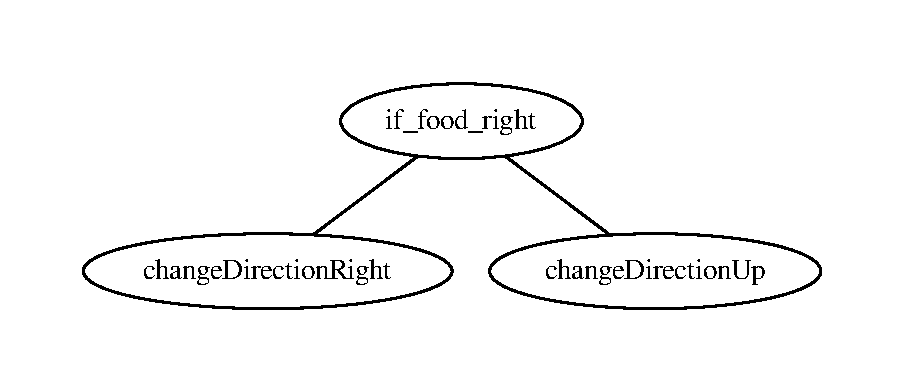
\includegraphics[width=0.7\linewidth]{figures/tree}
		\caption{Example tree representation of an individual.}
		\label{fig:tree}
	\end{figure}
	
	\begin{table}[]
		\centering
		\begin{tabu} to \textwidth {|X[l]|X[l]|}
			\hline
			changeDirectionDown, changeDirectionLeft, changeDirectionRight, changeDirectionUp & Changes the direction the snake is facing. \\  
			\hline
			nothing & The snake remains in the same direction.  \\  
			\hline
		\end{tabu}
		
		\caption{Terminal function set}
		\label{table:terminals}
	\end{table}
	
	Two different non-terminal sets were considered. The first one defines food, wall and tail sensing in all four direction relative to the grid. This set will be referred to as the absolute non-terminal set and can be see on \autoref{table:absolute-non-terminals}
	
	\begin{table}[h!]
		\centering
		\begin{tabu} to \textwidth {|X[3,l]|X[5,l]|}
			\hline
			if\_food\_up(o1, o2), if\_food\_down(o1, o2), if\_food\_left(o1, o2), if\_food\_right(o1, o2) & If there is food in the line/column of squares to the end of the grid in the specified direction execute first argument otherwise execute second argument\\  
			\hline
			
			if\_wall\_up(o1, o2), if\_wall\_down(o1, o2), if\_wall\_left(o1, o2), if\_wall\_right(o1, o2) & If there is a wall in the square to the specified direction execute first argument otherwise execute second argument\\  
			\hline
			
			if\_tail\_up(o1, o2), if\_tail\_down(o1, o2), if\_tail\_left(o1, o2), if\_tail\_right(o1, o2) & If there is part of the snake's body in the square to the specified direction execute first argument otherwise execute second argument\\  
			\hline
			
			prog2(o1, o2) & Executes its first argument, then executes second argument \\   
			\hline
		\end{tabu}
		
		\caption{Relative non-terminal function set}
		\label{table:relative-non-terminals}
	\end{table}
	
	The second non-terminal set defines the sensing functions relative to the snake's direction of travel. Because the movements are defined in terms of the absolute direction, useful routines cannot be constructed. For example, if there is danger on the left of the snake, it does not know in which direction relative to the grid it has to turn to avoid it. For this reason, additional sensing functions are added, which determine the direction in which the snake is travelling. Furthermore, the snake's body will always be behind it so there is no need to include sensing for what is behind. This function set will be referred to as the relative non-terminal set (see \autoref{table:relative-non-terminals}).
	
	\begin{table}[h!]
		\centering
		\begin{tabu} to \textwidth {|X[3,l]|X[5,l]|}
			\hline
			if\_food\_ahead(o1, o2), if\_food\_on\_left(o1, o2), if\_food\_on\_right(o1, o2) & If there is food in the line/column of squares to the end of the grid on the specified side of the snake execute first argument otherwise execute second argument\\  
			\hline
			
			if\_wall\_ahead(o1, o2), if\_wall\_on\_left(o1, o2), if\_wall\_on\_right(o1, o2) & If there is a wall in the square on the specified side of the snake execute first argument otherwise execute second argument\\  
			\hline
			
			if\_tail\_ahead(o1, o2), if\_tail\_on\_left(o1, o2), if\_tail\_on\_right(o1, o2) & If there is part of the snake's body in the square on the specified side of the snake execute first argument otherwise execute second argument\\  
			\hline
			
			if\_moving\_up(o1, o2), if\_moving\_down(o1, o2), if\_moving\_left(o1, o2), if\_moving\_right(o1, o2) & If the snake is moving in the specified direction execute first argument otherwise execute second argument\\  
			\hline
			
			prog2(o1, o2) & Executes its first argument, then executes second argument \\   
			\hline
		\end{tabu}
		
		\caption{Absolute non-terminal function set}
		\label{table:absolute-non-terminals}
	\end{table}
	
	This type of representation was chosen because it naturally maps the agents operators to the individual in the GP algorithm. As opposed to using an EA to find some meta parameters for an agent's controller, this approach makes solutions understandable and easier to analyse. It has been successfully applied to the snake game \cite{ehlis_application_2000} and the Santa Fe Ant problem \cite{koza_genetic_1992}. A possible downside to this representation might be the large function set. A large function set might require a substantial amount of computational resources to find a solution if the fitness landscape is rough.
	
	\subsection{Fitness evaluation}
	Two different fitness functions were considered and experimented with. The first one (see \autoref{eq:1}) is just the number of food items the snake eats during a single run (the score). 
	
	\begin{equation} \label{eq:1}
		Fitness = score
	\end{equation}
	
	The second fitness function considered, is the sum of the score and the total number of moves the snake has made during the run. In addition, the snake's fitness is penalised if it has died because it has not eaten any food for 196 moves. This fitness function can be seen in \autoref{eq:2}. where $steps$ is the total number of moves the snake has made, $timer=196$ and $I(timerExpired)$ is a boolean function such that $I(timerExpired) = 1$ if $timerExpired=True$ and $I(timerExpired)=0$ otherwise. $TimerExperied$ is true if the snake has made 196 moves without eating any food.
	
	\begin{equation} \label{eq:2}
		Fitness = score + steps - I(timerExpired) * timer
	\end{equation}
	
	The choice of the second evaluation function was motivated by the fact that the Hamiltonian \autoref{fig:ham_path} path solutions do not explicitly aim for the food. A possible way to motivate individuals to tend towards such a solution, is to give the higher fitness for traversing the grid. Nevertheless, there has to be a trade-off between the pursue of food and the number of moves made. In earlier generations individuals would tend to go in a loop in order to maximise the $steps$. In order to ensure this does not happen, the penalty is introduced.
	
	\subsection{Evolution operators and parameters}
	In \autoref{table:parameters} the evolution operators and parameters are given. They either arise from the problem domain or were found empirically. Population size and number of generations were highly restricted by the computational resources available, but were set to as high values as possible.  

	\begin{table}[h!]
		\centering
		\begin{tabu} to \textwidth {|X[l]|X[l]|}
			\hline
			Population size & 600 \\ \hline  
			Number of generations & 400  \\ \hline 
			Crossover rate & 0.6  \\ \hline  
			Mutation rate & 0.1  \\ \hline    \hline
			
			Initialisation & Ramped half and half \\ \hline
			Initialise min depth & 2  \\ \hline  
			Initialise max depth & 9  \\ \hline  \hline 
			
			Selection & Selection double tournament \\ \hline
			Tournament size & 7  \\ \hline  
			Parsimony size & 1.2  \\ \hline  \hline
			
			Crossover  &  One point crossover with leaf bias \\ \hline
			Leaf crossover probability & 0.1  \\ \hline
			
			Mutation & 	Uniform \\ \hline
			Mutation tree initialisation & Full \\ \hline
			Mutation Min Depth & 1  \\ \hline  
			Mutation Max Depth & 2  \\ \hline  \hline
			
			Bloat control & Static limit on number tree nodes \\ \hline
			Max Nodes & 150  \\ \hline  
			Hall of fame size & 1 \\ \hline
		\end{tabu}
		
		\caption{Evolution operators and parameters}
		\label{table:parameters}
	\end{table}
	
	\subsubsection{Initialisation}
	For the initialisation of individuals the ramped half and half method \cite{koza_genetic_1992} is used. It was chosen in order to increase diversity in the initial population. The maximum depth was determined empirically. There cannot be a useful tree with depth one, so the minimum was set to 2. Although, in most cases initialisation produces a good initial population, in some cases bloat occurs, even with bloat control in place (see \autoref{subsubsec:bloat}), because of the high maximum tree depth. However, it had to be set to a high enough value, in order to encourage diversity.
	
	\subsubsection{Selection}
	Initially a simple selection tournament was used as the selection operator. However, in order to limit bloat, a selection double tournament was chosen later on. Tournament size was chosen empirically and based on computational resources available. The parsimony size was set to relatively small value, in order not to discourage diversity.
	
	\subsubsection{Crossover}
	The crossover operator was chosen based on the specific problem - applying crossover to the leaf nodes in the tree essentially replaces one movement action with another. This can rarely lead to beneficial constructs in the offspring, but can lead to good solutions being destroyed. For this reason, crossover with a leaf node bias was used. The probability of choosing a leaf as a crossover point was set 0.1 and the probability of choosing a none leaf node - 0.9. The overall crossover rate was chosen empirically to be 0.6.
		
	\subsubsection{Mutation}
	The chosen mutation operator is uniform mutation and uses the full method to construct new trees. In this particular problem, mutations can often ruin existing solutions, rather than finding new ones. Furthermore, it is unlikely that randomly generated  trees of great depth would yield beneficial constructs. For this reason, the maximum depth of generated trees was set to 2 and the overall mutation probability of the algorithm to 0.1.  
	
	\subsubsection{Bloat control} \label{subsubsec:bloat}
	In order to mitigate the effects of bloat, a static limit on the number of nodes in each individual tree was used. This limit was applied to mutation and crossover, so any individual produced by the two operators, which had a grater number of nodes, was discarded. Limiting tree size was also necessary due to limited computation resources. There is also evidence that for the similar Santa Fe Ant problem, the proportion of solutions, in smaller trees, is higher \cite{langdon_why_1998}. 
	
	Limiting tree depth was also considered. However sparse deep trees were observed to have a high fitness in some cases. Also it is not clear what the depth limit should be set to without limiting the solution space. 
	
	Although, the size limit is applied to crossover  and mutation, it is not applied to initialisation, meaning that bloat can still occur. However, it is much more unlikely to occur, because of the size limit and the double selection tournament, which favours smaller individuals.

    % 4) Results [35 marks]
	\section{Results} \label{results}
	Three versions of the algorithm were compared to determine the best one. They use a different combination of the above mentioned function sets and evaluation functions \autoref{table:algorithms}. 
	
	First algorithms 1 and 2 will be compared, followed by a comparison of 1 and 3. 
	
		\begin{table}[h!]
			\centering
			\begin{tabu} to \textwidth {|X[1l]|X[2l]|X[2l]|X[1l]|}
				\hline
				\textbf{Algorithm} & \textbf{Evaluation Function} & \textbf{Function set} & \textbf{parameters} \\ \hline
				
				Algorithm 1  & Composite (\autoref{eq:2}) & Absolute non-terminals (\autoref{table:absolute-non-terminals}) and terminals (\autoref{table:terminals})  &  from \autoref{table:parameters}\\ \hline  
				
				Algorithm 2  & Simple (\autoref{eq:1}) & Absolute non-terminals (\autoref{table:absolute-non-terminals}) and terminals (\autoref{table:terminals})  &  from \autoref{table:parameters}\\ \hline  
				
				Algorithm 3  & Composite (\autoref{eq:2}) & Relative non-terminals (\autoref{table:relative-non-terminals}) and terminals (\autoref{table:terminals})  &  from \autoref{table:parameters}\\ \hline  
			\end{tabu}
			
			\caption{Algorithms}
			\label{table:algorithms}
		\end{table}
		
		\subsection{Algorithm evaluation} \label{subsec:evaluation}
		Each algorithm was ran 20 times. The best individual for each run was recorded and evaluated 100 times. In order to perform a fair comparison between algorithms, the random seed was fixed, for each of the evaluation runs, to the run number(from 0 to 99). This means that the food in the game environment was placed in the same positions for each pair of runs with the same random seed. 
		
		\subsection{Experimental results} \label{subsec:results}
		On \autoref{fig:score_vs_size} the average score and size for each algorithm is shown. Comparing algorithm 1 (\autoref{fig:alg1_score_vs_size}) with algorithms 2 (\autoref{fig:alg2_score_vs_size}) and 3 \autoref{fig:alg3_score_vs_size}, it achieves a much higher score than the others. Furthermore, the average size of algorithm 1's tree is the lowest. This could be an indication that the proportion of good solution is higher in smaller tree sizes as suggested by \cite{langdon_why_1998}.
		
		Algorithm 2 converges the fastest out of the three and it's average size starts off close to the limit of 150 in early generations and goes down in later generations. The fast convergence can be accounted to the simpler fitness function. Agents quickly learn to pursue the food, but since their fitness does not incorporate staying alive for longer, they do not adapt to avoid danger.
		
		Algorithm three achieves similar results to algorithm 2 in terms of the score achieved, however the average tree size is much larger than any of the others. In fact the size is above the size limit of 150, which indicates that bloat has occurred in several runs.
		
		
		\begin{figure}[h!]
			\begin{subfigure}{.33\textwidth}
			\centering
			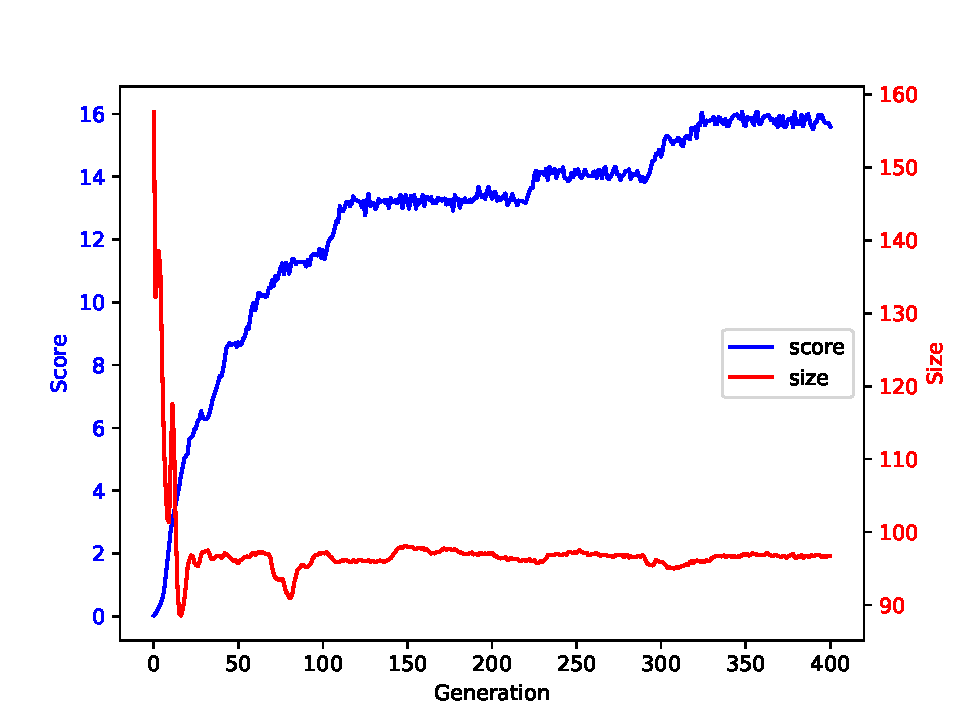
\includegraphics[width=\linewidth]{../code/plots/alg1_score_vs_size}
			\caption{Algorithm 1}
			\label{fig:alg1_score_vs_size}
			\end{subfigure}
			\begin{subfigure}{.33\textwidth}
			\centering
			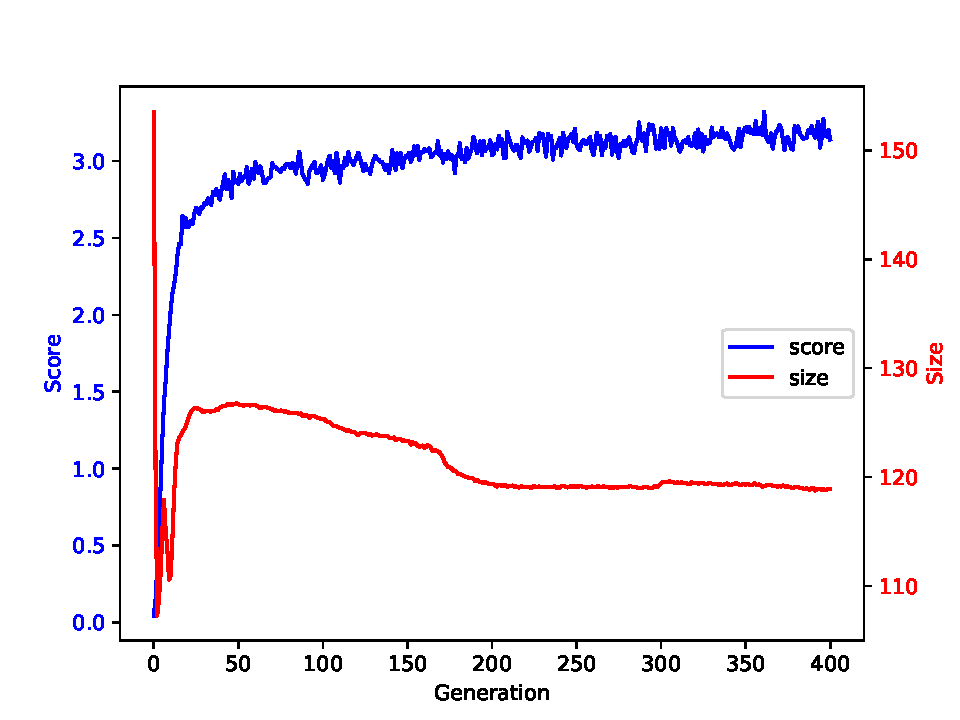
\includegraphics[width=\linewidth]{../code/plots/alg2_score_vs_size}
			\caption{Algorithm 2}
			\label{fig:alg2_score_vs_size}
			\end{subfigure}
			\begin{subfigure}{.33\textwidth}
			\centering
			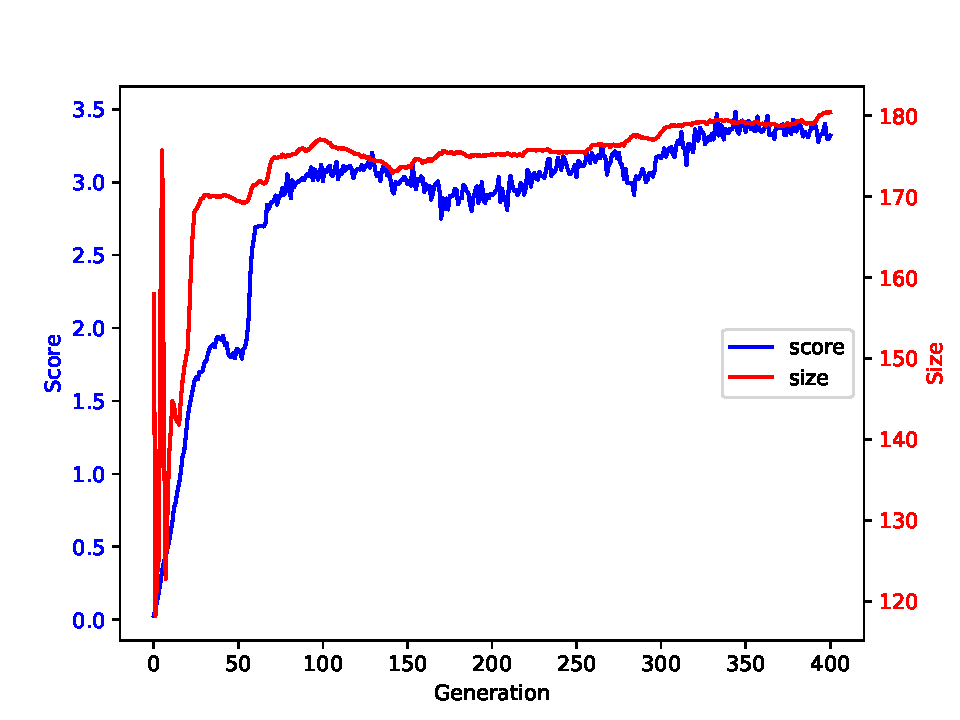
\includegraphics[width=\linewidth]{../code/plots/alg3_score_vs_size}
			\caption{Algorithm3}
			\label{fig:alg3_score_vs_size}
			\end{subfigure}
			
			\caption{Average score and average size for each generation out of 20 runs.}
			\label{fig:score_vs_size}
		\end{figure}
		
		In figures \autoref{fig:alg1_score}, \autoref{fig:alg2_score} and \autoref{fig:alg3_score} the maximum and minimum scores are shown in addition to the average. The minimum score for all three algorithms is 0, which is to be expected as mutation and crossover can often destroy good individuals. The maximum scores achieved however are much more comparable with algorithm 1 having the best one followed by 3 and 2.
		
		\begin{figure}[h!]
			\begin{subfigure}{.33\textwidth}
				\centering
				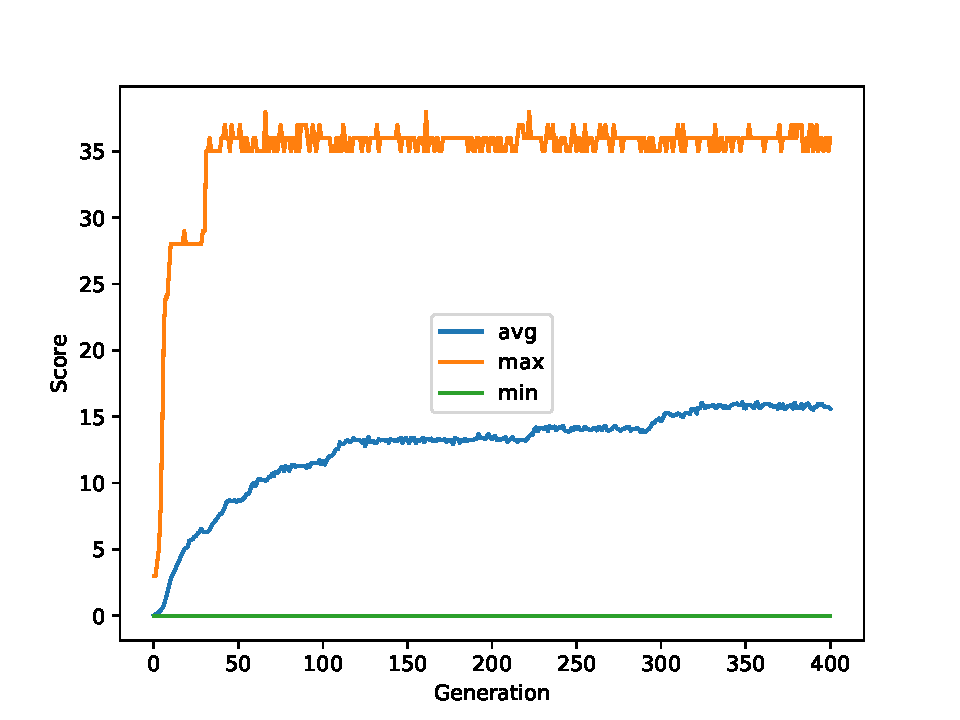
\includegraphics[width=\linewidth]{../code/plots/alg1_score}
				\caption{Algorithm 1}
				\label{fig:alg1_score}
			\end{subfigure}
			\begin{subfigure}{.33\textwidth}
				\centering
				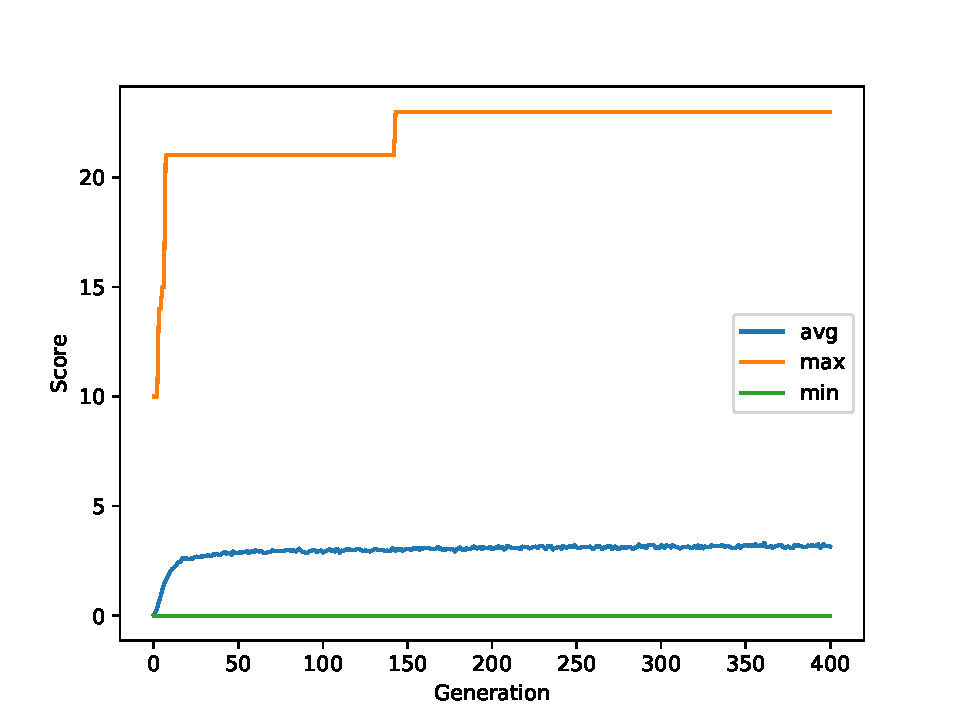
\includegraphics[width=\linewidth]{../code/plots/alg2_score}
				\caption{Algorithm 2}
				\label{fig:alg2_score}
			\end{subfigure}
			\begin{subfigure}{.33\textwidth}
				\centering
				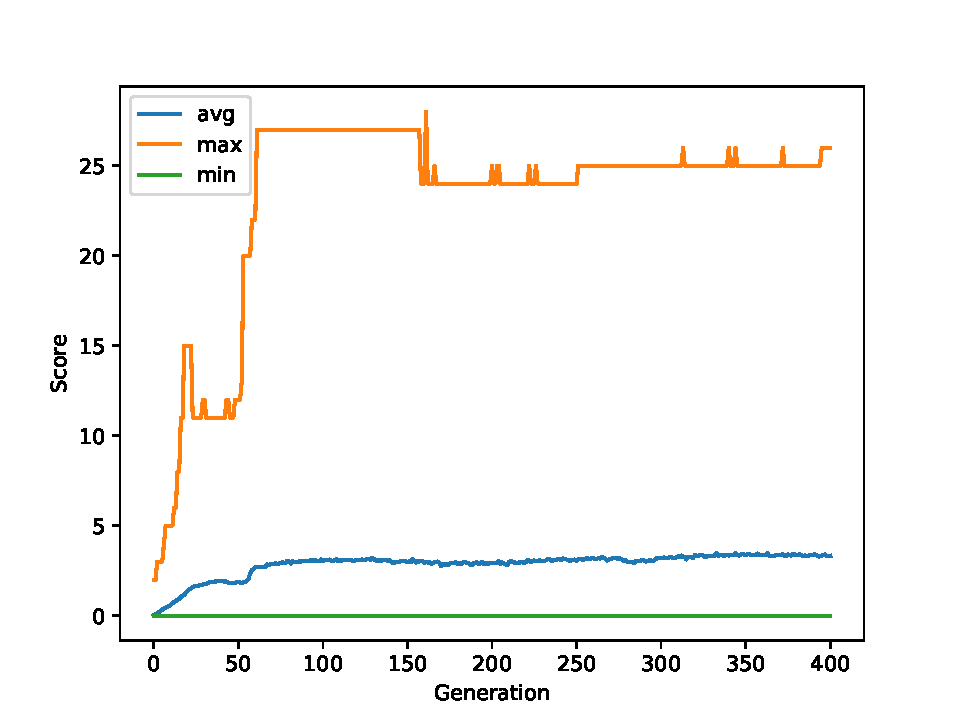
\includegraphics[width=\linewidth]{../code/plots/alg3_score}
				\caption{Algorithm3}
				\label{fig:alg3_score}
			\end{subfigure}
			
			\caption{Average maximum and minimum score for each generation out of 20 runs.}
			\label{fig:score}
		\end{figure}
		Figures \autoref{fig:alg1_bests_dist}, \autoref{fig:alg2_bests_dist} and \autoref{fig:alg3_bests_dist} show the distribution of the best 20 individuals out of all runs over their average scores on the test problems. These scores were obtaained on the same set of 100 problems (see \autoref{subsec:evaluation}) and therefore are most reliable for comparing the three algorithms. Looking at the plots we see that for each algorithm there is a single best individual outlier. The distributions of algorithms 2 and 3 are very skewed and look almost identical. On the other hand the distribution of algorithm 1 is more spread out. Also, almost half of the individuals from algorithm 1 seem to outperform the individuals from algorithms 2 and 3.
		
		In order to find out if there is a significant difference in the distributions a Mann–Whitney U test was conducted. The results of the test for each pair of algorithms can be seen in \autoref{table:u-test}. The p-values for algorithm 1 and 2 and 1 and 3 are below the threshold of 0.05. This means that the null hypothesis that the sample for algorithm 1 comes from the same distribution as the other two samples. However this is not true for algorithms 2 and 3 since the p-value for them is much higher than the threshold of 0.15.
		
		
		\begin{figure}[h!]
			\begin{subfigure}{.33\textwidth}
				\centering
				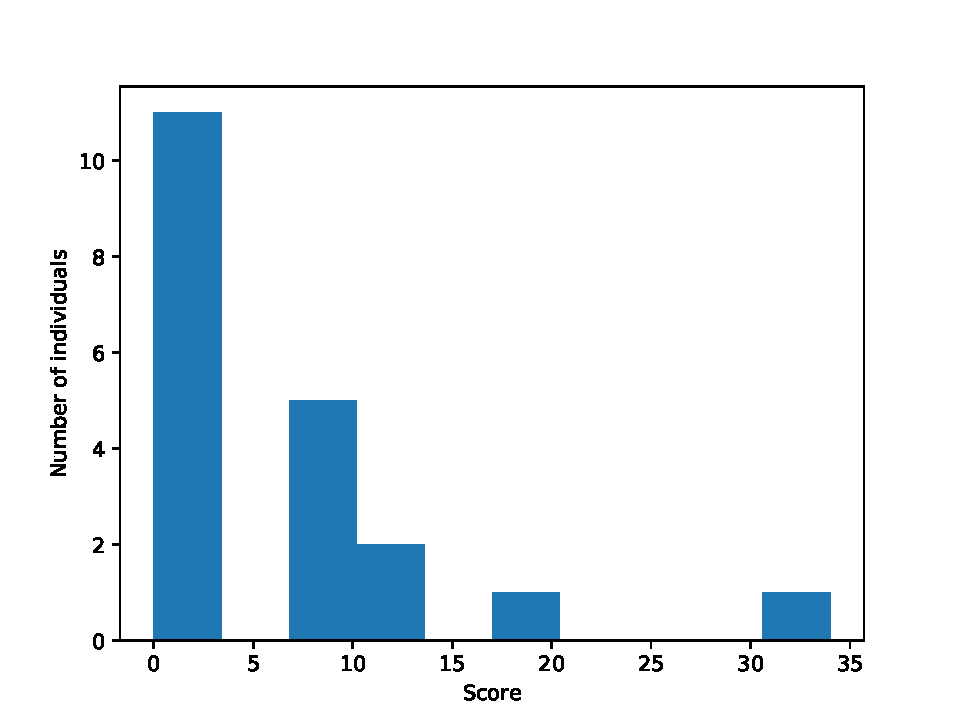
\includegraphics[width=\linewidth]{../code/plots/alg1_bests_dist}
				\caption{Algorithm 1}
				\label{fig:alg1_bests_dist}
			\end{subfigure}
			\begin{subfigure}{.33\textwidth}
				\centering
				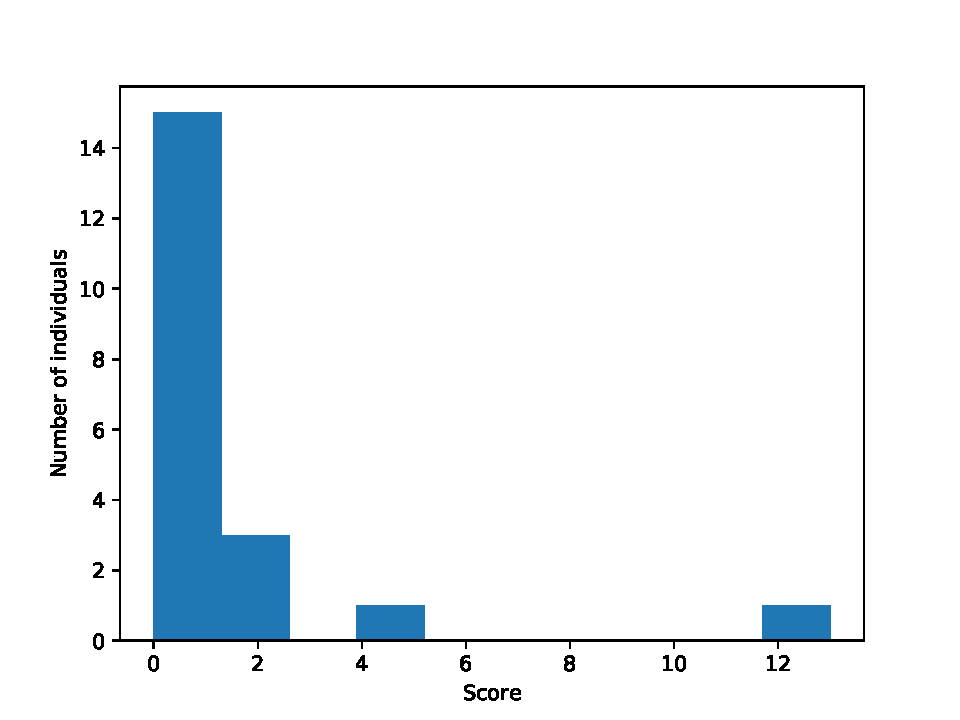
\includegraphics[width=\linewidth]{../code/plots/alg2_bests_dist}
				\caption{Algorithm 2}
				\label{fig:alg2_bests_dist}
			\end{subfigure}
			\begin{subfigure}{.33\textwidth}
				\centering
				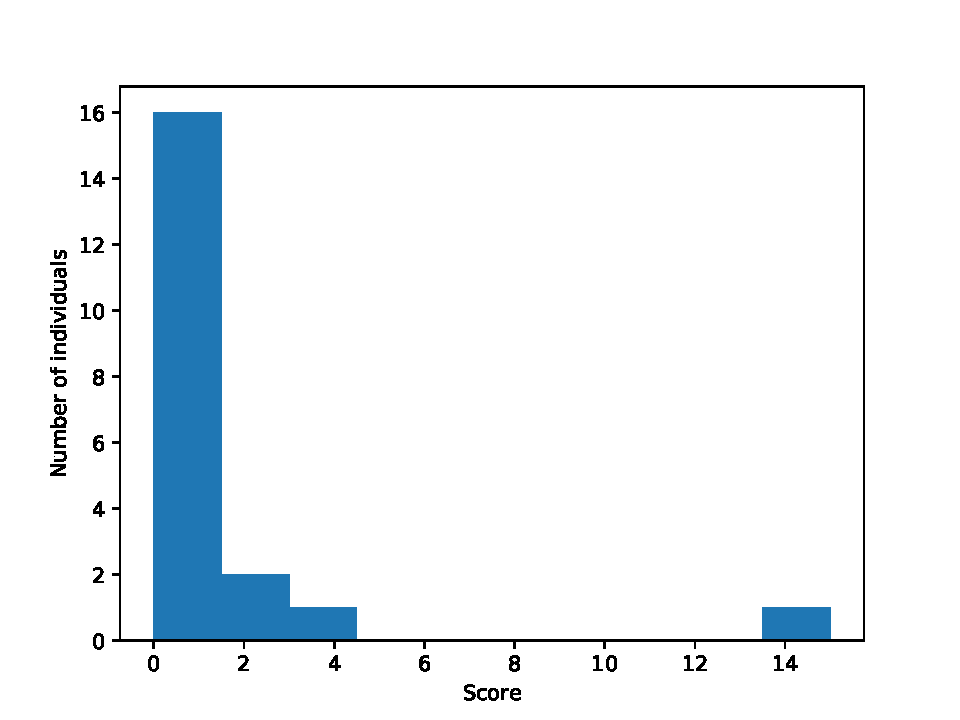
\includegraphics[width=\linewidth]{../code/plots/alg3_bests_dist}
				\caption{Algorithm3}
				\label{fig:alg3_bests_dist}
			\end{subfigure}
			
			\caption{Distribution of individuals evaluated on 100 test runs over their average score.}
			\label{fig:bests_dist}
		\end{figure}
		
		
		\begin{table}[h!]
			\centering
			\begin{tabu} to \textwidth {|X[l]|X[l]|X[l]|}
				\hline
				\textbf{First algorithm} & \textbf{Second algorithm} & \textbf{p-value} \\ \hline
				Algorithm 1 & Algorithm 2 & 0.0038075456551803864 \\ \hline
				Algorithm 1 & Algorithm 3 & 0.0010537832718209305 \\ \hline
				Algorithm 2 & Algorithm 3 & 0.15610108279449836   \\ \hline
			\end{tabu}
			
			\caption{Mann–Whitney U test results}
			\label{table:u-test}
		\end{table}	
		
		Finally, looking at \autoref{fig:alg1_best_dist}, \autoref{fig:alg2_best_dist} and \autoref{fig:alg3_best_dist}, a comparison between the single best individuals,from all 20 runs of each algorithm, can be made. For about 50\% of the runs, algorithm 1 has achieved a score of around 35. However, the distribution is bimodal and has the largest spread out of all algorithms.
		
		
		\begin{figure}[h!]
			\begin{subfigure}{.33\textwidth}
				\centering
				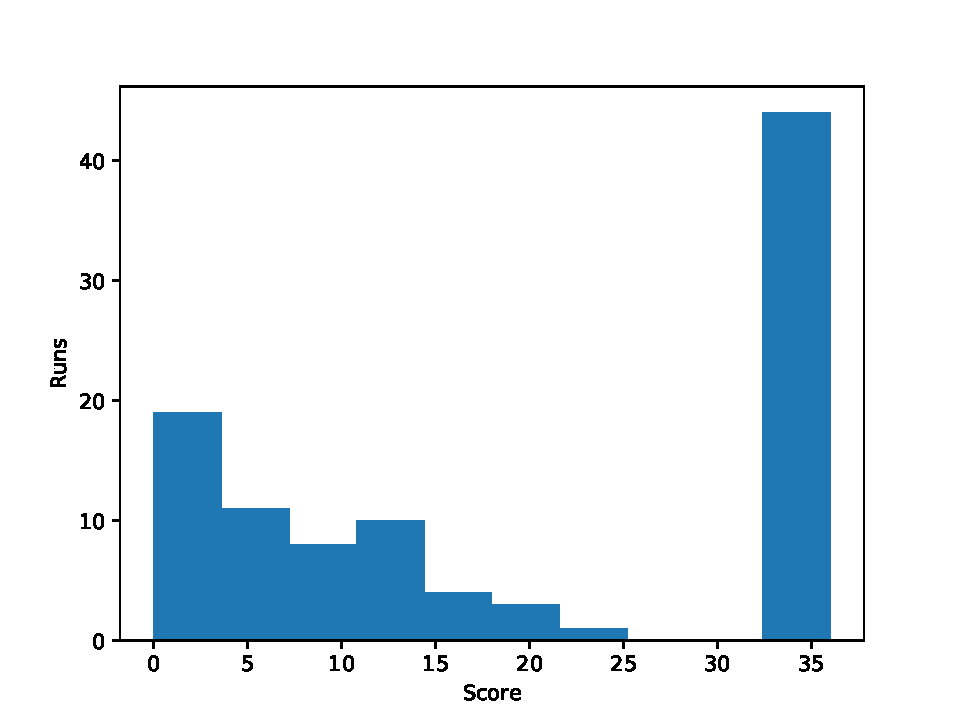
\includegraphics[width=\linewidth]{../code/plots/alg1_best_dist}
				\caption{Algorithm 1}
				\label{fig:alg1_best_dist}
			\end{subfigure}
			\begin{subfigure}{.33\textwidth}
				\centering
				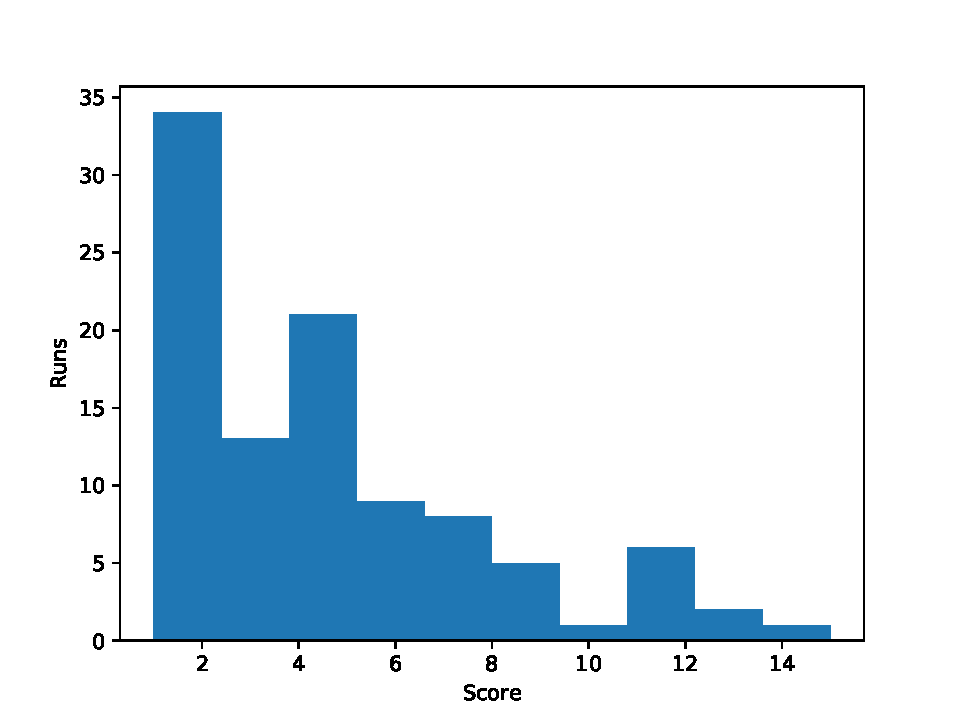
\includegraphics[width=\linewidth]{../code/plots/alg2_best_dist}
				\caption{Algorithm 2}
				\label{fig:alg2_best_dist}
			\end{subfigure}
			\begin{subfigure}{.33\textwidth}
				\centering
				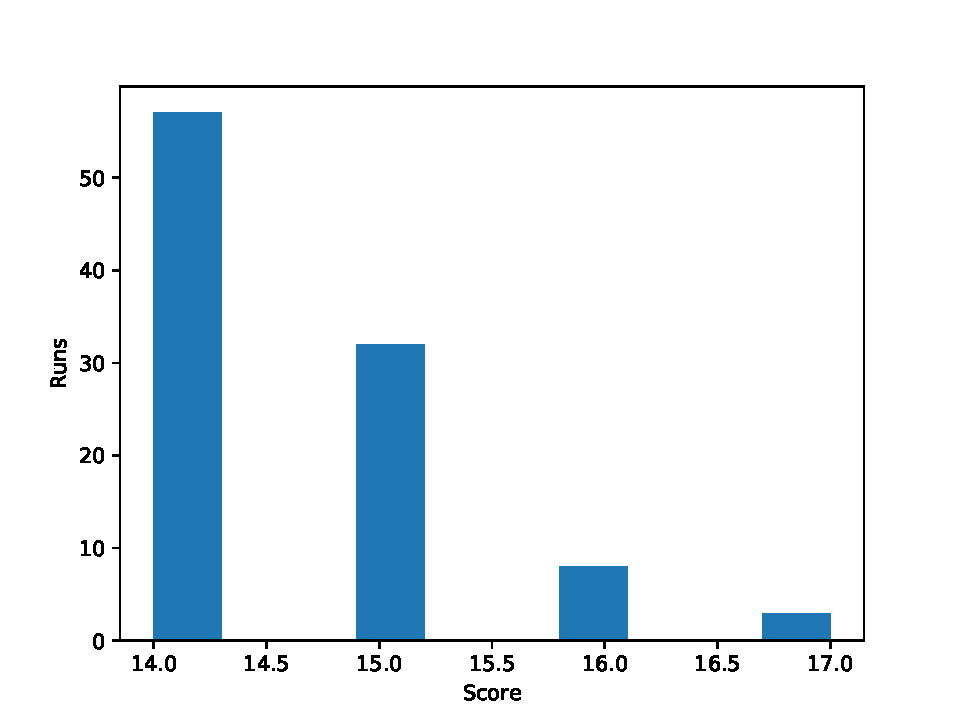
\includegraphics[width=\linewidth]{../code/plots/alg3_best_dist}
				\caption{Algorithm3}
				\label{fig:alg3_best_dist}
			\end{subfigure}
			
			\caption{Distribution of results for 100 evaluations of the single best individual.}
			\label{fig:best_dist}
		\end{figure}
		
		
		

		

    % 5) Conclusions [10 marks]
	\section{Conclusion} \label{conclusions}
	
	key points
	representation may be shit
	hamiltonian path not achieved
	
	connection with snake paper
	potential connection with size stuff
	
	
	
	\subsection{Future Work}
	more computation
	iterative method from paper
	mmix between non terminals
	
	NOTE ADD REFS TO STATS

	\printbibliography
	
	\appendix
	
\end{document}